\documentclass{standalone}
\usepackage{tikz}
\usepackage{ctex,siunitx}
\setCJKmainfont{Noto Serif CJK SC}
\usepackage{tkz-euclide}
\usepackage{amsmath}
\usetikzlibrary{patterns, calc,3d}
\usetikzlibrary {decorations.pathmorphing,decorations.pathreplacing,decorations.shapes}
\begin{document}
\small
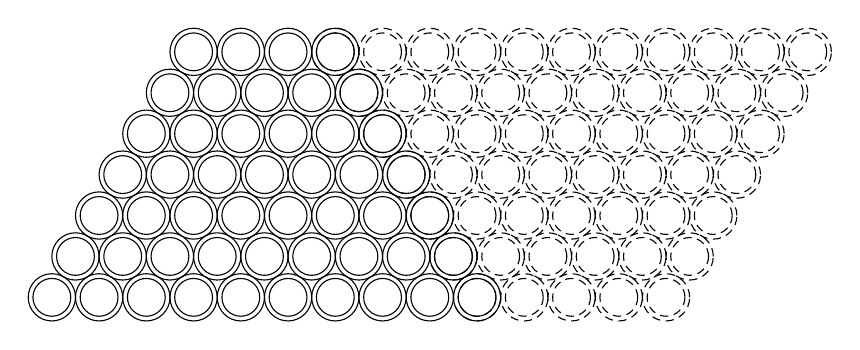
\begin{tikzpicture}[>=latex,scale=0.6]
  \foreach \r[count=\i from 0] in {3,4,...,9}
  {
    \foreach \x in {0,1,...,\r}
    {
      \draw([xshift=\x cm]-120:\i)circle(0.5);
      \draw([xshift=\x cm]-120:\i)circle(0.4);
    }
    \foreach \x in {\r,...,13}
    {
      \draw[densely dashed]([xshift=\x cm]-120:\i)circle(0.5);
      \draw[densely dashed]([xshift=\x cm]-120:\i)circle(0.4);
    }
  }
\end{tikzpicture}
\end{document}